\newpage

\section*{\centerline{Цель работы}}

Получение навыков работы с командной строкой UNIX и UNIX-подобных систем, а также навыки работы с файлами: просмотр редактирование, поиск и архивирование в GNU/Linux. Изучить основные команды и утилиты, поработать с правами на файлы и директории в GNU/LINUX. 
\newpage

\section*{\centerline{Выполнение}}
	\vspace{1cm}

	\subsection*{\centerline{Часть 1}}
		Задачи:\\
		1) Изучение команд для скачивания файлов из Интернета.\\
		2) Изучение команд для работы с архивами.\\
		3) Изучение команд для поиска файлов и слов в файлах.\\
		\vspace{1cm}
		\\

		\paragraph*{1.1)Скачивание файлов из интернета с использованием терминала\\\\}
		Цель:Дан список ссылок (текстовый файл в приложении). Проверить доступность файлов по ссылке. \\

		Команда \textit{wget --spider url} позволяет проверить доступность файла по указанному адресу url.\\
		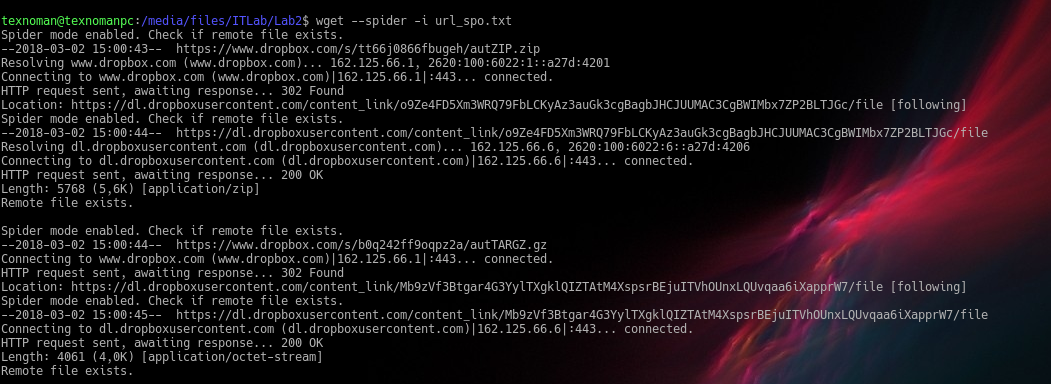
\includegraphics [width=\textwidth]{picture1.png}\\
		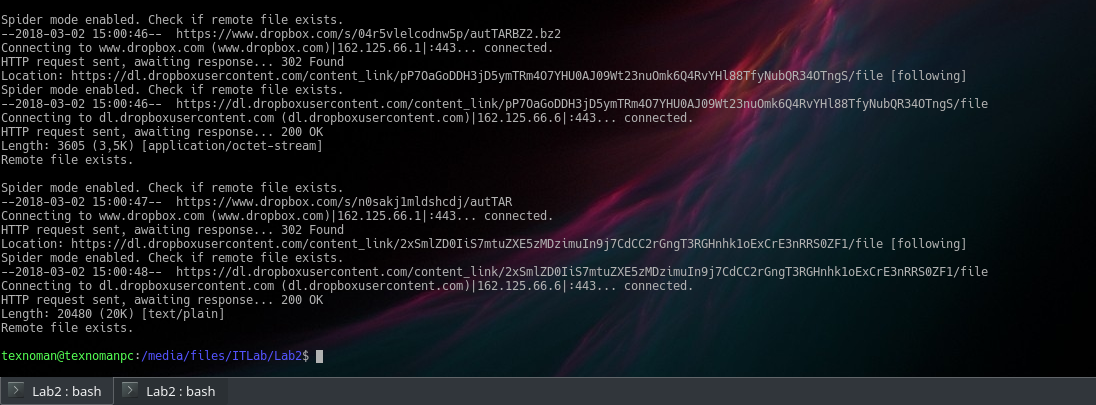
\includegraphics [width=\textwidth]{picture2.png}\\
		\vspace{0.5cm}
		\\
		Цель:Скачать первый в списке доступный файл, не меняя его имя.\\

		Команда \textit{wget -i filename} позволяет скачать файл по ссылке из файла. Ключик \textit{-i} значит, что мы берем список \textit{url} из файла С помощью \textit{head -n 1} можно получить первую строку файла. Значок \textit{<} переводит вывод построчно в активный поток ввода\\
		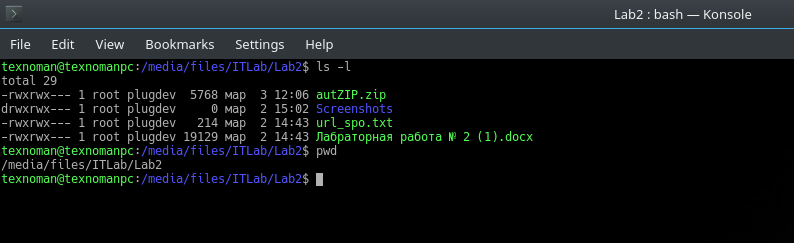
\includegraphics [width=\textwidth]{picture3.png}\\
		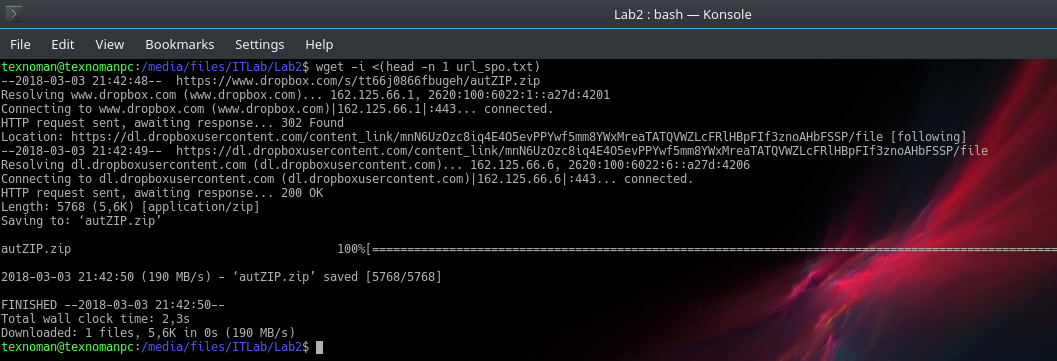
\includegraphics [width=\textwidth]{picture4.png}\\
		\vspace{0.5cm}
		\\
		Цель: Скачать второй доступный файл в lab2, изменив его имя на var1\\

		Скачивание файла по второй ссылке из файла. Также используется \textit{sed}, но забирает он уже вторую строку при помощи ключика \textit{-n '2p'}\\
		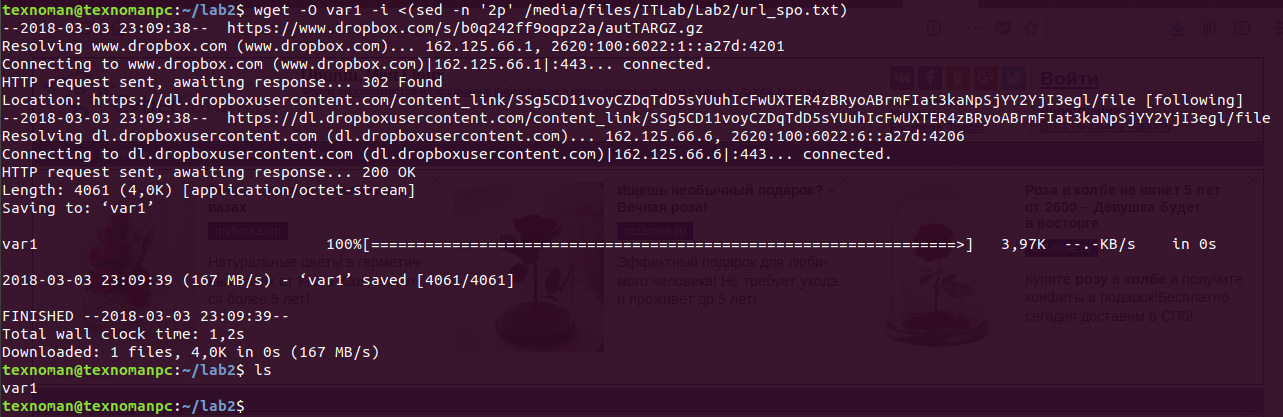
\includegraphics [width=\textwidth]{wget(var1).png}\\
		\\
		Цель:Остальные доступные файлы докачать из текстового файла в директорию lab2.\\

		Выборку остальных файлов можно осуществить при помощи команды \textit{sed} способной во входящем потоке отредактировать файл и удалить не нужные нам строки. Удаление строк происходит с помощью специального выражения 
		\textit{1,2d}\\
		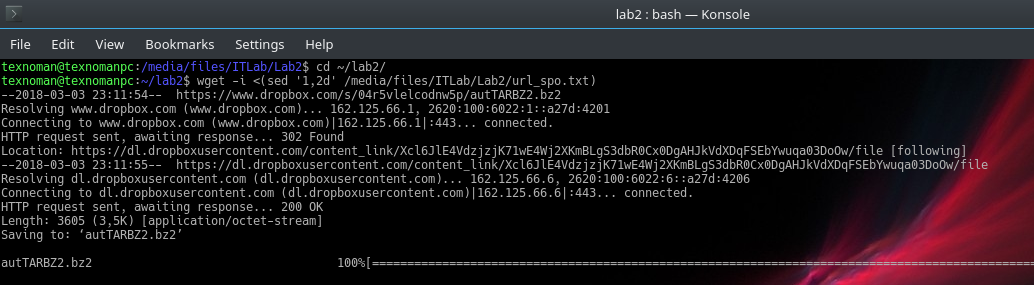
\includegraphics [width=\textwidth]{picture5.png}\\
		\vspace{0.5cm}
		\\
		Цель:Выбрать любой сайт про Лермонтова. Скачать все .jpeg, .jpg файлы с сайта. Установить глубину  = 1. Объяснить работу команды. Показать результат\\

		Скачивание всех \textit{.jpeg}, \textit{.jpg} файлов с сайта про Лермонтова. Используется глубина рекурсии 1 (ключик \textit{-l1}). Не создаются поддиректории(ключик \textit{-nd}) Ключик \textit{-А} необходим для построчного разделения полученных url.\\\
		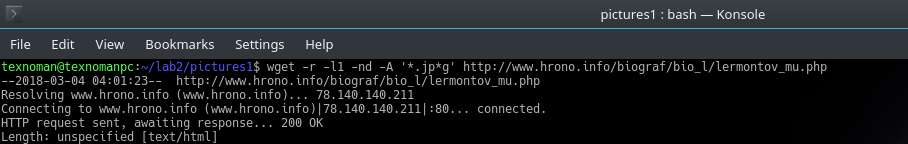
\includegraphics [width=\textwidth]{picture6.png}\\
		\begin{center}
			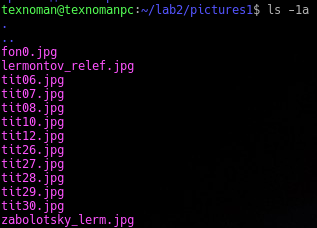
\includegraphics [width=0.7\textwidth]{pictures9.png}\\
		\end{center}
		\vspace{1cm}
		


		\paragraph*{1.2) Работа с архивами\\\\}
		
		Цель: Проверка формата файлов(архивов).\\

		Используется Команда \textit{file}, но можно использовать и \textit{ls --mimetype}\\
		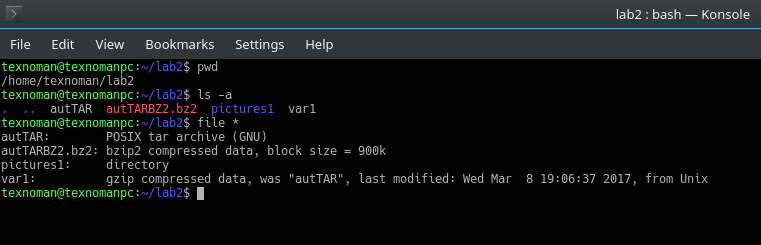
\includegraphics [width=\textwidth]{picture10.png}\\
		\vspace{0.5cm}
		\\
		Цель: Из .zip архива извлечь файл \textit{Лермонтов.txt}\\

		Извлечение из \textit{.zip} архива файла Лермонтов.txt Используется утилита \textit{unzip}\\
		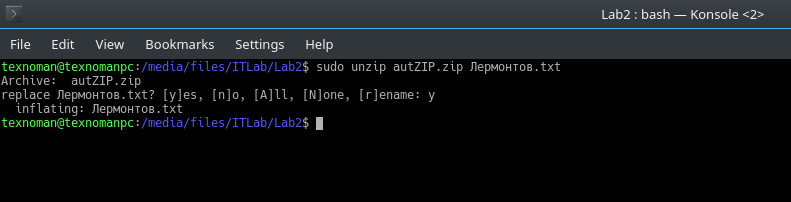
\includegraphics [width=\textwidth]{picture22.png}\\
		\vspace{0.5cm}
		\\
		Цель:Архивы .tar, .tar.gz, .tar.bz2 распаковать с выводом информации о процессе на экран\\

		Распаковка архивов \textit{.tar, .tar.gz, .tar.bz2} с выводом информации о процессе на экран (необходим ключик -v: verboose)\\
		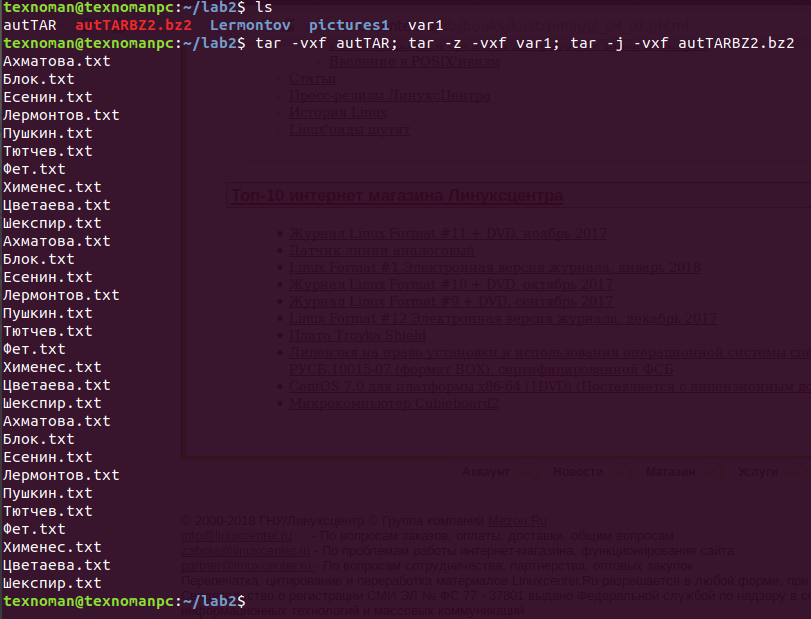
\includegraphics [width=\textwidth]{tar(3).png}\\
		\vspace{0.8cm}


		\paragraph*{1.3) Поиск файлов, поиск по тексту\\\\}
		
		Цель: Найти все файлы, созданные в домашней папке за последний день:\\

		Нахождение всех файлов, созданных за последний 1 дней в домашней папке. Так как их было много, содержимое вывода не влезло в окно консоли\\
		
\includegraphics [width=\textwidth]{picture23.png}\\
		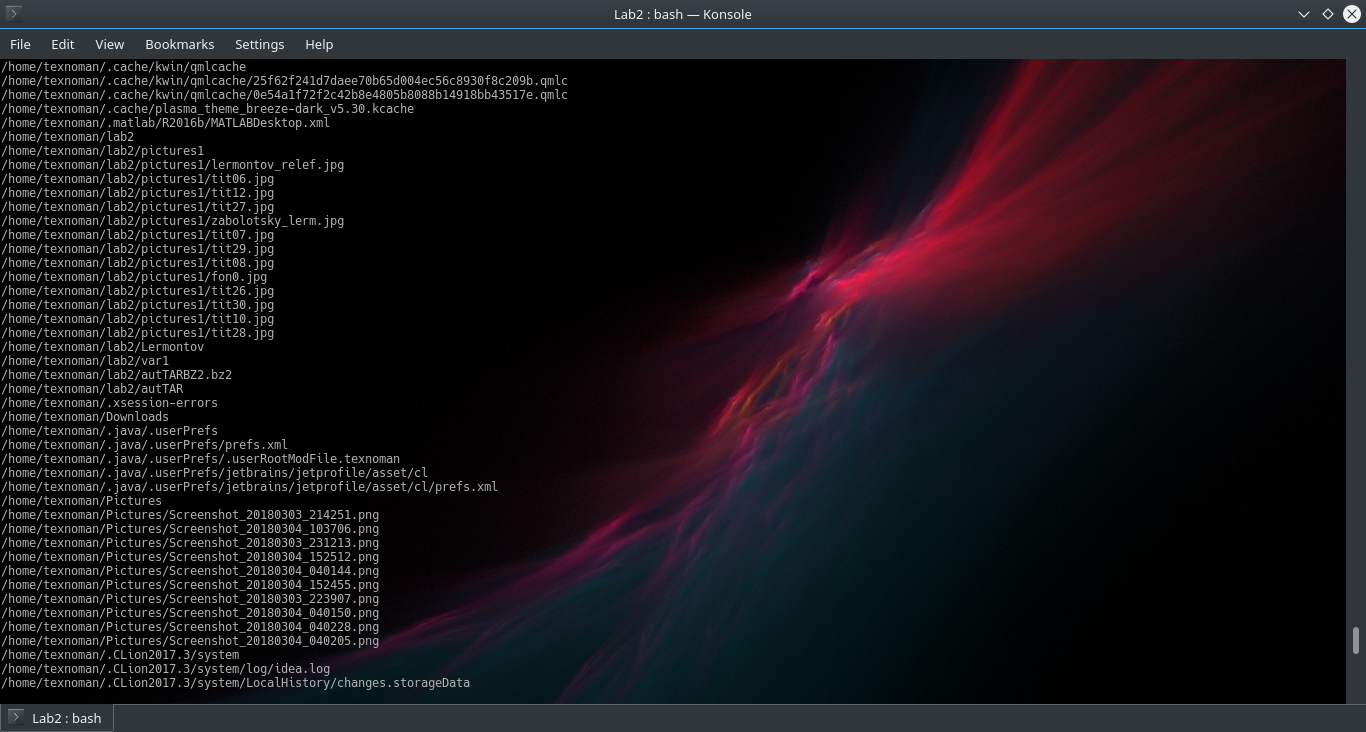
\includegraphics [width=\textwidth]{picture12.png}\\
		\vspace{0.5cm}
		\\
		Цель: Найти все файлы c фамилией автора автора\\

		Нахождение всех файлов с фамилией Лермонтов с использованием команда \textit{find}, способной искать файлы по маске или регулярному выражению\\
		
\includegraphics [width=\textwidth]{find_Lermontov.png}\\
		\vspace{0.5cm}
		\\
		Цель: Переместить файлы с произведениями автора в папку /home/username/lab2/Произведение Лермонтова. Туда же переместить картинки.\\

		Перемещение этого файла в папку \textit{Произведения Лермонтова}. Перемещение туда же файлов с картинками из сайта о Лермонтове\\
		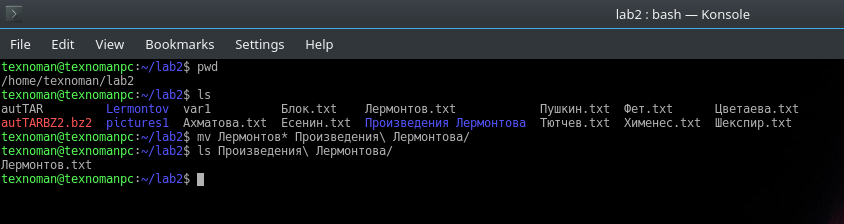
\includegraphics [width=\textwidth]{picture14.png}\\
		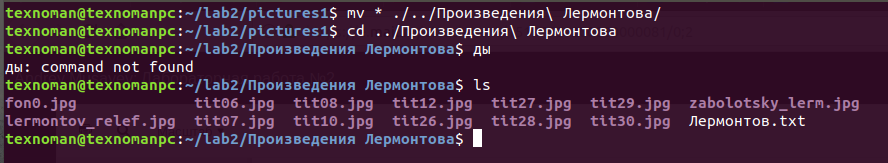
\includegraphics [width=\textwidth]{101.png}\\
		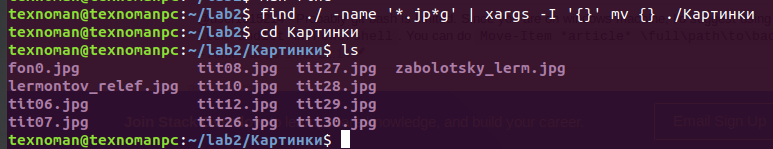
\includegraphics [width=\textwidth]{102.png}\\
		\vspace{0.5cm}
		\\
		Цель: Найти  .jpg и .jpeg файлы, скаченные в п. 7. Задания 1. Переместить файлы с картинками в папку /home/username/lab2/Картинки\\

		Смена кодировки файла \textit{Лермонтов.txt} c \textit{windows-1251} на \textit{Unicode}. Используется команда 
		\textit{iconv}\\
		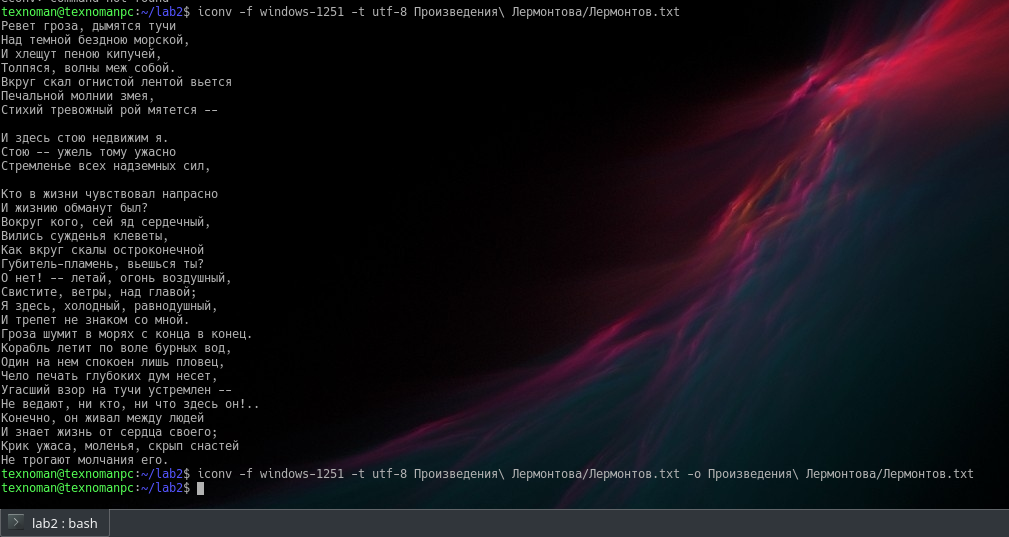
\includegraphics [width=\textwidth]{picture16.png}\\
		\vspace{0.5cm}
		\\
		Цель: Найти слова в файлах \textit{я, то?} и посчитать количество совпадений. Примечание: ?, * - спец. символы\\

		Поиск слов \textit{я, то?} (\textit{?}- является спец. символом) в файле, подсчет строк может быть осуществлен при использовании ключа \textit{-c}\\
		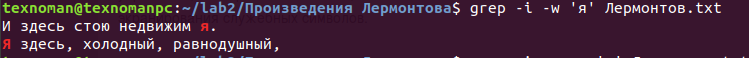
\includegraphics [width=\textwidth]{103.png}\\
		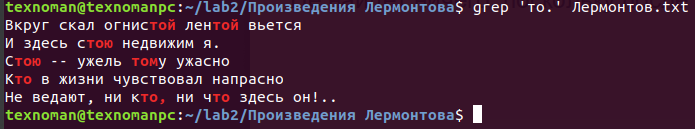
\includegraphics [width=\textwidth]{119.png}\\
		\vspace{1cm}
		\\
		Цель: Посчитать количество строк/ слов/ символов (см. табл., столб.4) в файлах с произведениями.\\

		Посчет количества строк в файлах с произведениями. Было решено использовать команду \textit{grep}, способную работать с регулярными выражениями\\
		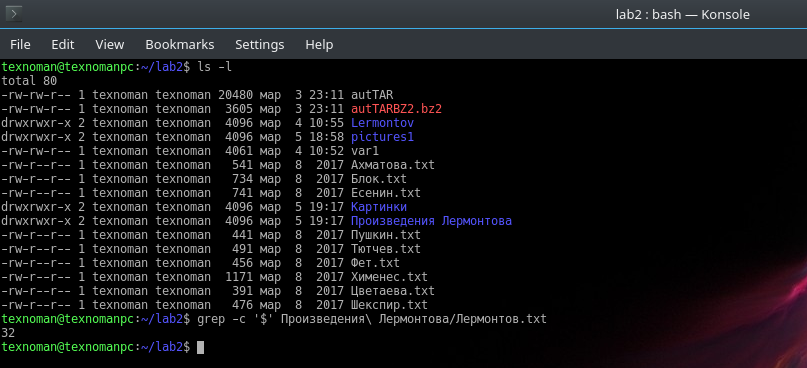
\includegraphics [width=\textwidth]{picture17.png}\\
		\vspace{0.5cm}

		\paragraph*{1.4) Работа с архивами(архивирование)\\\\}

		Цель:Папку «Произведение автора» и «Картинки» заархивировать (Без удаления исходных папок!!!) в три архива типов: .zip , .tar (использовать вывод на экран информации о процессе архивирования), .tar.gz (запаковать архив с использованием ровно одной команды терминала).\\

		Архивирование папок "Произведения Лермонтова" и "Картинки" в \textit{tar ,zip} и \textit{tar} сжатый \textit{gz}
		Для сжатия  и параллельной запаковки при помощи \textit{gz} использовать tar с ключиком \textit{-z}. Ключик 
		\textit{-c} необходим для создания архива(create). Ключик \textit{-f} необходим для включения в архив содержимого файлов. Ключик \textit{-v} позволяет вывести подробную информацию о запаковке или распаковке.
		\\
		\begin{center}
			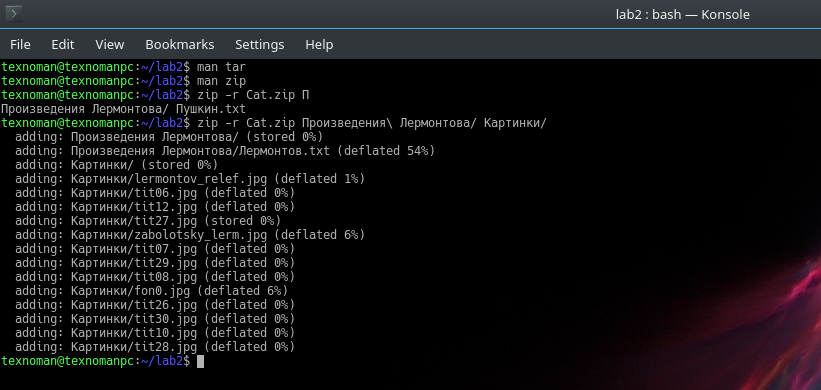
\includegraphics [width=\textwidth]{picture18.png}\\
			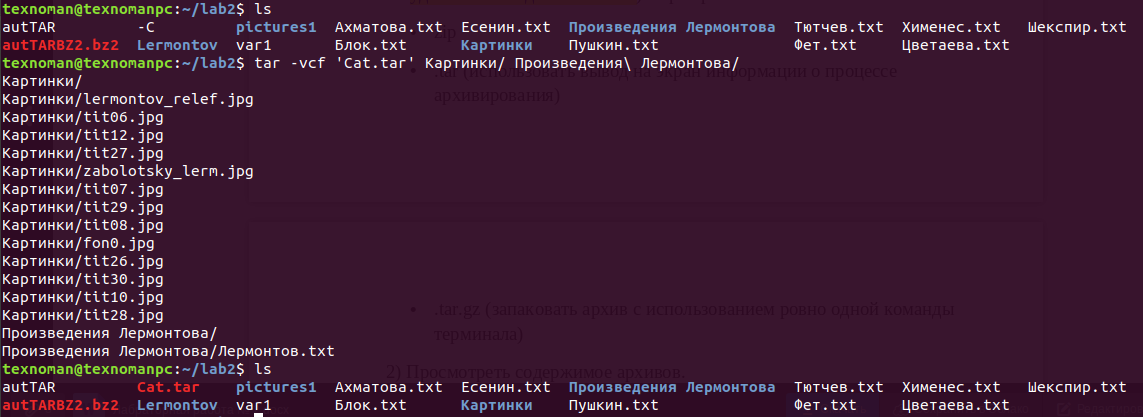
\includegraphics [width=\textwidth]{106.png}\\
			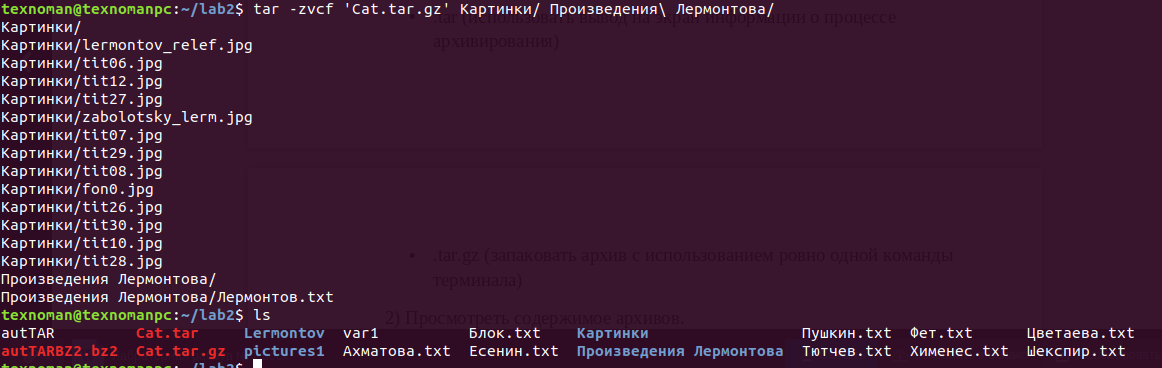
\includegraphics [width=\textwidth]{107.png}\\
		\end{center}
		\vspace{0.5cm}
		
		Цель: проверка содержимого архива.\\
		
		Проверка архивирования. Проверяем содержимое архивов при помоши спец. ключа \textit{-t} для архивов tar и при помощи \textit{zipinfo} для zip \\
		\begin{center}
			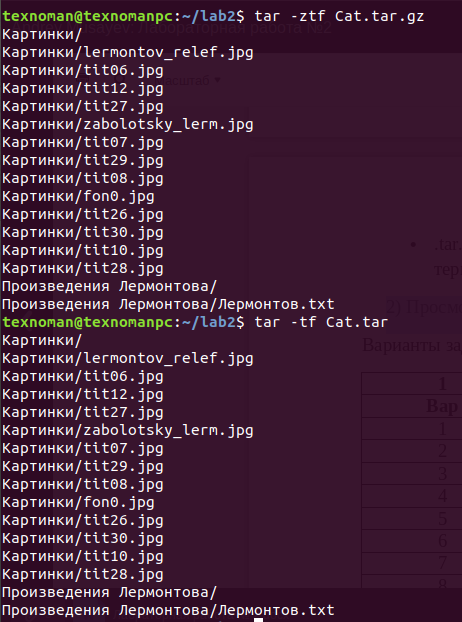
\includegraphics [width=0.5\textwidth]{109.png}\\
			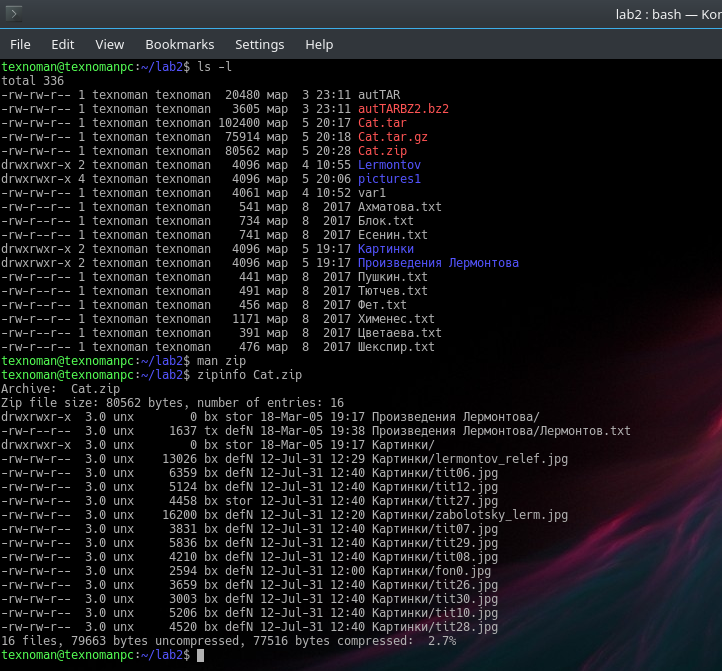
\includegraphics [width=\textwidth]{picture19.png}\\
		\end{center}
		
		\vspace{0.5cm}


